% Configuration
%===============================================================================
% Zentrale Layout-Angaben und Befehle
%===============================================================================
%
% Für bessere Sicht von falschen Umbrüchen die Option draft benutzen.
% Dadurch können aber die eingebundenen Bilder nicht sichtbar sein.
\documentclass[a4paper, 12pt]{article}
%
% Hier zunächst die benötigten Packages
\usepackage[utf8]{inputenc}
\usepackage{fancyhdr}
\usepackage[T1]{fontenc}
\usepackage{ae}
\usepackage{listings}
\usepackage{color}
\usepackage{listings}
\usepackage{wrapfig}
\usepackage[printonlyused]{acronym}
\usepackage{url}
\usepackage{hyperref}
\usepackage{multirow}
\usepackage{float}
\usepackage{afterpage}
\usepackage{tabularx}

\newcommand\blankpage{%
	\null
	\thispagestyle{empty}%
	\addtocounter{page}{1}%
	\newpage}
%\usepackage{svg}
%
% Einbindung des Grafik-Pakets
\ifx\pdfoutput\undefined
	\usepackage[dvips]{graphicx}
\else
	\usepackage[pdftex]{graphicx}
\pdfcompresslevel=9
\pdfpageheight=297mm
\pdfpagewidth=210mm
\fi
%
% Page-Layout
\setlength\headheight{14pt}
\setlength\topmargin{-15,4mm}
\setlength\oddsidemargin{-0,4mm}
\setlength\evensidemargin{-0,4mm}
\setlength\textwidth{160mm}
\setlength\textheight{252mm}
%
% Absatzeinstellungen
\setlength\parindent{0mm}
\setlength\parskip{2ex}
%
% Kopf- und Fusszeile
\pagestyle{fancy}
\fancyhf{} % alles löschen
\fancyhead[LO]{\footnotesize\sc\nouppercase{\leftmark}}
\fancyfoot[LO]{\footnotesize\sc Distributed Systems Group}
\fancyfoot[RO]{\thepage}
\renewcommand{\headrulewidth}{0pt}
\renewcommand{\footrulewidth}{0pt}
%
% Bessere Fehlermeldungen
\errorcontextlines=999
%
% Anweisung zur Erstellung der Titelseite
% #1 Bachelorarbeit || Masterarbeit
% #2 = Studiengang
% #3 = Titel der Arbeit
% #4 = Autor
% #5 = Abgabedatum
\renewcommand{\maketitle}[5]
{
\pagenumbering{Alph}
\begin{titlepage}
\centering
\begin{minipage}[t]{16cm}
\begin{minipage}{3cm}
    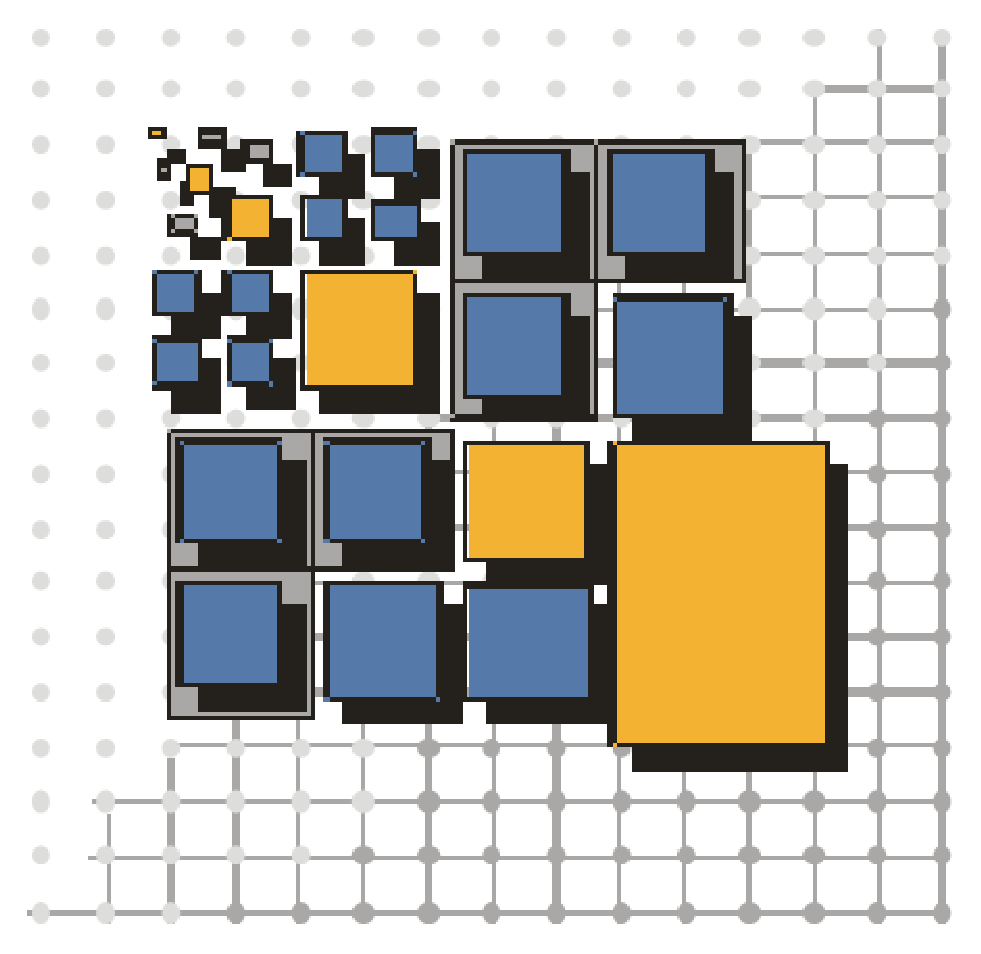
\includegraphics[height=26mm]{includes/vs-logo}
\end{minipage}
\hfill
\begin{minipage}{9cm}
  \centering
    University of Bamberg\\[12pt]
    {\Large Distributed Systems Group}
\end{minipage}
\hfill
\begin{minipage}{3cm}
    
\includegraphics[height=26mm]{includes/UB-Logo-neu_blau-cmyk}
\end{minipage}
\end{minipage}\\[130pt]
{\LARGE #1}\\[24pt]
in the degree programme #2\\
at the Faculty of Information Systems and Applied Computer Sciences,\\ University of Bamberg\\[90pt]
Topic:\\[24pt]
{\Huge #3}\\[60pt]
\vfill
\begin{minipage}{\textwidth}
\center
Author:\\
{\Large #4\\[12pt]}
Reviewer:\\
Prof. Dr. Guido Wirtz\\[12pt]
Date of submission:\\
#5\\
\end{minipage}
\end{titlepage}
}
%
% Anweisung zur Erstellung der Eigenständigkeitserklärung
% #1 = Typ der Arbeit
% #2 = Datum
% #3 = Vorname Name
\newcommand{\makedeclaration}[3]
{
	\fancyhead[LO]{\footnotesize\sc\nouppercase{Declaration}}
	%
			\vspace*{16cm}
			In accordance with § 9 Para. 12 APO, I hereby declare that I wrote the preceding #1 independently and did not use any sources or aids other than those indicated. Furthermore, I declare that the digital version corresponds without exception in content and wording to the printed copy of the #1 and that I am aware that this digital version may be subjected to a software-aided, anonymised plagiarism inspection.
			\vspace*{1cm}
			
			Bamberg, #2 \hspace{5cm} #3
	%
}
%
% Wird für Hintergrund von Codelistings benötigt
\definecolor{hellgrau}{gray}{0.9}
%
% Einstellungen für Java-Code
\lstdefinestyle{javaStyle}{%
	basicstyle=\small,%
	backgroundcolor=\color{hellgrau},%
	keywordstyle=\bfseries,%
	showstringspaces=false,%
	numbers=left,%
	numberstyle=\footnotesize,%
	stepnumber=1,%
	numbersep=3pt,%
	extendedchars=true,%
	xleftmargin=2em,%
	lineskip=-1pt,%
	tabsize=4,%
	language=Java,
	breaklines,%
	identifierstyle=\ttfamily,
}
%
% neues environment für Java-Sourcecode
% #1 = "caption={Hier eigene Überschrift}, label={Hier eigenes Label}"
\lstnewenvironment{javacode}[1][]{%
\lstset{style=javaStyle,#1}%
}{}
%
% Befehl zum Einbinden von Java-Sourcecode aus Datei
% #1 = Dateiname relativ zu src-Verzeichnis
% #2 = Überschrift
% #3 = Label
\newcommand{\javafile}[3]{%
   \lstinputlisting[%
     caption={#2},%
     label={#3},%
     style=javaStyle]{src/#1}%
}
%
% Einbindung eines Bildes
% #1 = label für \ref-Verweise
% #2 = Name des Bildes ohne Endung relativ zu images-Verzeichnis
% #3 = Beschriftung
% #4 = Breite des Bildes im Dokument in cm
\newcommand{\asfigure}[4]{%
  \begin{figure}[htb]%
    \begin{center}%
      \includegraphics[width=#4cm]{images/#2}%
      \vskip -0.3cm%
      \caption{#3}%
      \vskip -0,2cm%
      \label{#1}%
    \end{center}%
  \end{figure}%
}
%
% Umgebung für Fliesstext um Grafik
% #1 = Ausrichtung: r, l, i, ...
% #2 = Breite des Bildes in cm
% #3 = Name des Bildes ohne Endung relativ zu images-Verzeichnis
% #4 = Beschriftung
% #5 = label für \ref-Verweise
\newcommand{\textflow}[5]{%
\begin{wrapfigure}{#1}{#2cm}%
\includegraphics[width=#2cm]{images/#3}%
\caption{#4}%
\label{#5}%
\end{wrapfigure}%
}
%%% Local Variables:
%%% mode: latex
%%% TeX-master: t
%%% End:

%
\begin{document}
%
% Titlepage
\maketitle{Master Thesis}{International Software Systems Science}{Open‐Source Software Discovery and Vulnerability Analysis}{Rajendran, Hari Prashanth}{01.10.2021}
%
% TOCs
\pagenumbering{Roman}
\tableofcontents
\newpage
\listoffigures
\newpage
\listoftables
\newpage
\lstlistoflistings
\newpage
\fancyhead[LO]{\footnotesize\sc\nouppercase{Abbreviations}}
%
% Abkürzungen
%
\section*{Abbreviations}
% In Klammern steht das längste Akronym!
\begin{acronym}[LSPI]
 \acro{DSG}{Distributed Systems Group}
 \acro{LSPI}{Lehrstuhl für Praktische Informatik}
 \acro{OSS}{Open-source Software}
 \acro{NVD}{National Vulnerability Database}
 \acro{CVE}{Common Vulnerabilities and Exposure}
 \acro{CPE}{Common Platform Enumeration}
 \acro{CVSS}{Common Vulnerability Scoring System}
 \acro{CERT/CC}{Computer Emergency Response Team Coordination Center}
 \acro{JSON}{JavaScript Object Notation}
 \acro{API}{Application Programming Interface}
 \acro{XML}{Extensible Markup Language}
\end{acronym}
\newpage
\fancyhead[LO]{\footnotesize\sc\nouppercase{\leftmark}}
\setcounter{page}{1}
\pagenumbering{arabic}
%
% Insert your chapters here
%
%
\section{Introduction}\label{sec:introduction}
%
Insert the text of your \acs{DSG} thesis here.
\subsection{Motivation}
Nowadays, firms and individuals are using different forms of computer software which is running on different platforms from a simple mobile application to a sophisticated distributed enterprise system. Even though the software is created using different methodologies based on a wide variety of technologies, still each has its own advantages and disadvantages \cite{tur38}\cite{KaDaPeTu2014}. Software security is an essential concern in the software development process because not only to reduce the additional cost but also it can cause severe damage for developers or organizations \cite{fil2}. In some recent years, there have been many incidents that happened in which software vulnerability imposed vital damage to companies and individuals. To make a clear idea of this issue, I have mentioned incidents that happened in recent years. A prominent example of open-source software vulnerability is the Equifax breach in 2017, which literally exposed 145 million users' data due to outdated open-source software. The outcome of this incident relies on openness because the same code has been seen by all users which includes the attackers\cite{WinNT}. Software vulnerabilities are imposed by the importance of the threats which depend on the factors like exploitation complexity and attack-surface[8]. Likewise, there have been a lot of incidents before in which the companies and individuals have been affected by software vulnerability with significant damage \cite{tur38}. In addition, vulnerabilities are common and fundamental. Therefore, choosing software is important to risk management for information security. Selecting software packages with strong security features can reduce risk management to individuals or organizations. \acs{OSS} has been referred to as a potential answer for software security issues and vulnerabilities because most of the open-source software licenses give full access to any part of the code to examine and modify \cite{KeJaSa2005}.

\subsection{Problem Statement}
In general open-source software is used massively in modern Software Development which says around 96\% of the application in the enterprise market uses open-source software. Today standard components are not re-written; instead they are shared as packages around the world. Open Source Portals like Github and Gitlab make it very easy to share those components. The advantage of this "Shared Code Culture" is also the biggest disadvantage because the whole Community and therefore also the components are constantly changing. Releases of components are often pushed daily if the project is active. But if the community switches or the main Authors are leaving, those projects become deprecated very fast. And due to rising IT security threats, a component can become insecure if not patched frequently. Whether an \acs{OSS} component will become critical also depends on the context where the component will be used. The context will define which actions need to be taken to use an \acs{OSS} component within the Project.  As opposed to these, I propose to build a scanner to extract all the possible open-source software components and their dependencies from software projects and perform data analysis with help of \acs{CVE} and \acs{NVD} to find the severity of each vulnerable component[6]. The very first challenge for building this scanner will be scanning for open-source software components and that should happen on the client-side of the system due to the source code privacy of the projects. Along with the scanning, the system should extract the open-source component meta information from a variety of software projects by using the best text analysis approach. After the extraction of the open-source software components, the next challenge will be assessing the vulnerability and its security issues of each component by choosing the right predictive analysis model. The final output of this scanning will be a PDF report which gives a clear detail of each open-source software component used inside the project.
\newpage
%
%
\section{Conclusion}\label{sec:conclusion}
%
This is the last chapter of this thesis \cite{tur38}.
%

%
\newpage
%
% References
\addcontentsline{toc}{section}{References}
\bibliographystyle{alpha}
%
% Insert your bibliography here
\bibliography{bibliography/references}
\newpage
%
% Eigenständigkeitserklärung APO
\makedeclaration{master’s thesis}{16.11.2012}{Alan Turing}
%
\end{document}
